% article example for classicthesis.sty
\documentclass[10pt,a4paper]{article} % KOMA-Script article scrartcl
\usepackage{import}
\usepackage{xifthen}
\usepackage{pdfpages}
\usepackage{transparent}
\newcommand{\incfig}[1]{%
    \def\svgwidth{\columnwidth}
    \import{./figures/}{#1.pdf_tex}
}
\usepackage{lipsum}     %lorem ipsum text
\usepackage{titlesec}   %Section settings
\usepackage{titling}    %Title settings
\usepackage[margin=10em]{geometry}  %Adjusting margins
\usepackage{setspace}
\usepackage{listings}
\usepackage{amsmath}    %Display equations options
\usepackage{amssymb}    %More symbols
\usepackage{xcolor}     %Color settings
\usepackage{pagecolor}
\usepackage{mdframed}
\usepackage[spanish]{babel}
\usepackage[utf8]{inputenc}
\usepackage{longtable}
\usepackage{multicol}
\usepackage{graphicx}
\graphicspath{ {./Images/} }
\setlength{\columnsep}{1cm}

% ====| color de la pagina y del fondo |==== %
\pagecolor{black}
\color{white}



\begin{document}
    %========================{TITLE}====================%
    \title{{  Notas tema 11 AED inferencias sobre la media de un vector  }}
    \author{{Rodrigo Castillo}}
    \date{\today}

    \maketitle


     % ====| Loguito |==== %
    
\includegraphics[width=0.1\linewidth]{negro_cara.png}
    %=======================NOTES GOES HERE===================%
    \section{caso univariado}
        para hacer una conclusion valida de la media de una muestra, si tienes
        p variables correlacionadas deben ser analizadas
        los test cubridos en este conjunto de notas son de la forma
        \begin{equation}
            \color{red}  H_o: \mu = \mu _o    \color{white}
        \end{equation}
        donde $ mu_{p \times 1}   $ es el vector de las medias poblacionales y
        $ \mu _{o,p \times 1}   $ son valores nulos en la hipótesis
        \\
        para el caso univariado...
        \begin{figure}[h!]
            \centering
            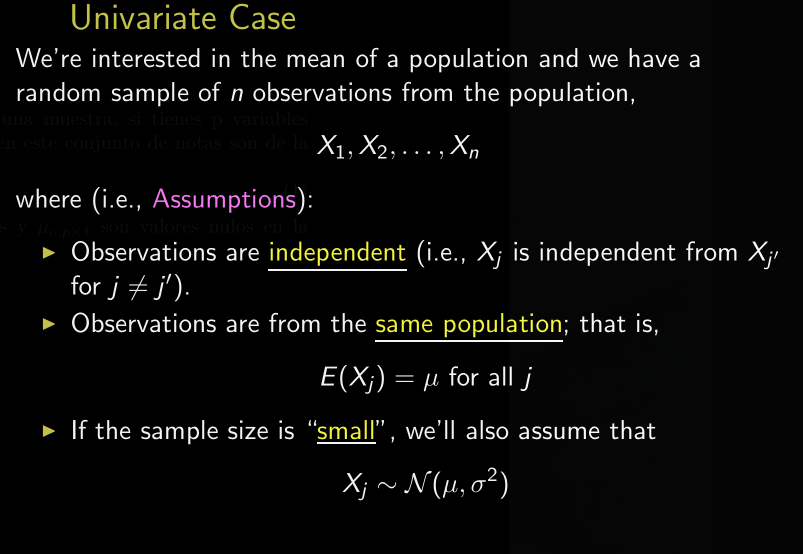
\includegraphics[width=0.8\linewidth]{univariado.png}
            \caption{Caso Univariado}
            \label{univariado}
        \end{figure}

        \newpage
        hipotesis y test ...

        \begin{figure}[h!]
            \centering
            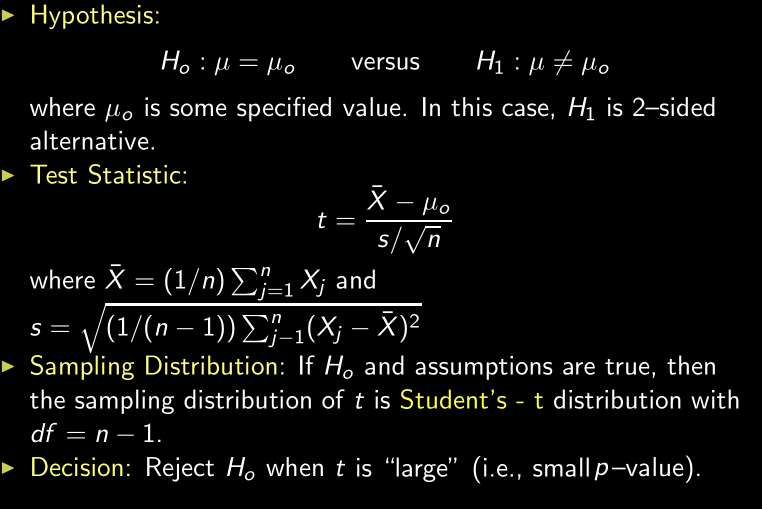
\includegraphics[width=0.8\linewidth]{hip.png}
            \caption{Hipotesis y test}
            \label{test}
        \end{figure}

        \newpage
        entonces la desicion es clasica para la distribucion $ t-student  $
        \begin{figure}[h!]
            \centering
            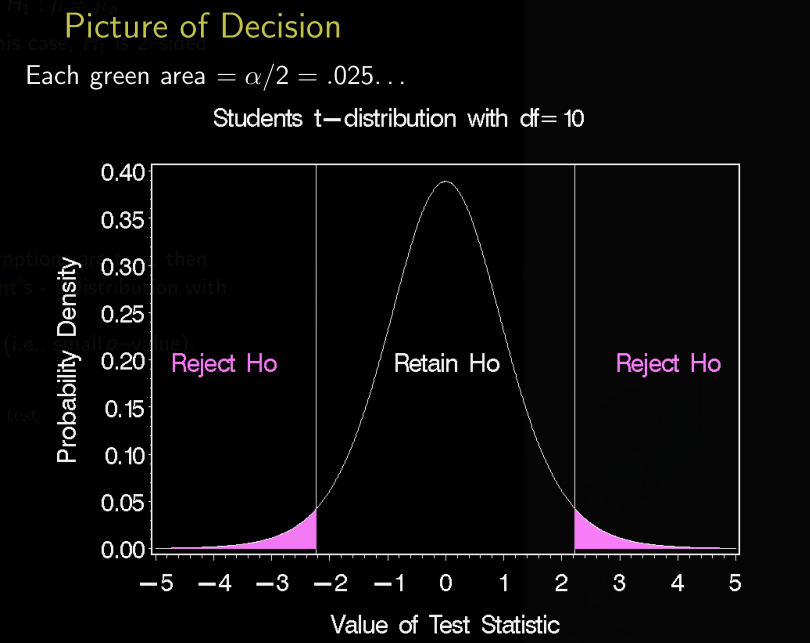
\includegraphics[width=0.8\linewidth]{des.png}
            \caption{Desición}
            \label{des}
        \end{figure}

        \newpage
        intervalos de confianza ...
        \\
        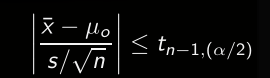
\includegraphics[width=0.8\linewidth]{conf.png}
        \\
        en donde $ T_{n-1}( \frac{\alpha }{2} )  $  es la parte superior $ blah
        blah blah...  $
        \begin{figure}[h!]
            \centering
            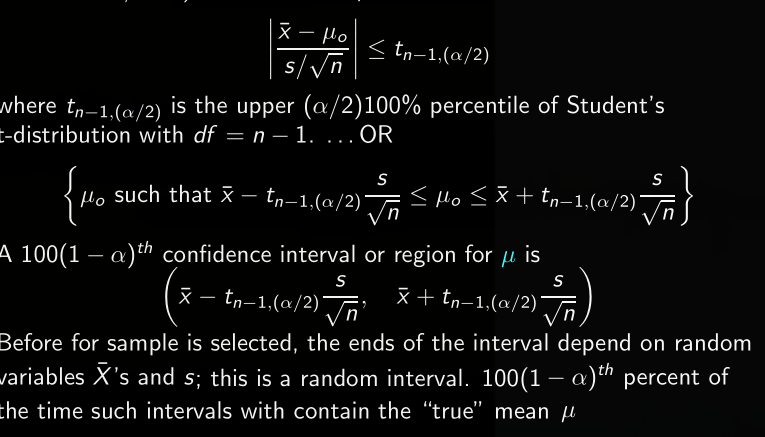
\includegraphics[width=0.8\linewidth]{test.png}
            \caption{Test}
            \label{fig}
        \end{figure}

    \section{caso multivariado}
        la extension del caso univariado, vamos a reemplazar los escalares para los vectores y matrices
        \\
        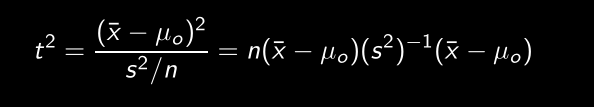
\includegraphics[width=0.8\linewidth]{t2.png}
        \\
        donde $ t ^{2}    $ es un metodo cuadrado estadistico de la distancia
        entre la muestra $ \hat{x}   $  y el valor hipotetico $ \mu _o  $

        se tiene que $ t_{df} ^{2}  = F_{1,df}  $


        eso quiere decir que la muestra de distribucion de
        \\
        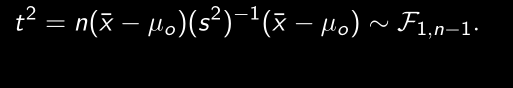
\includegraphics[width=0.8\linewidth]{tsample}
        \\
        y se extiende así ...

        \begin{figure}[h!]
            \centering
            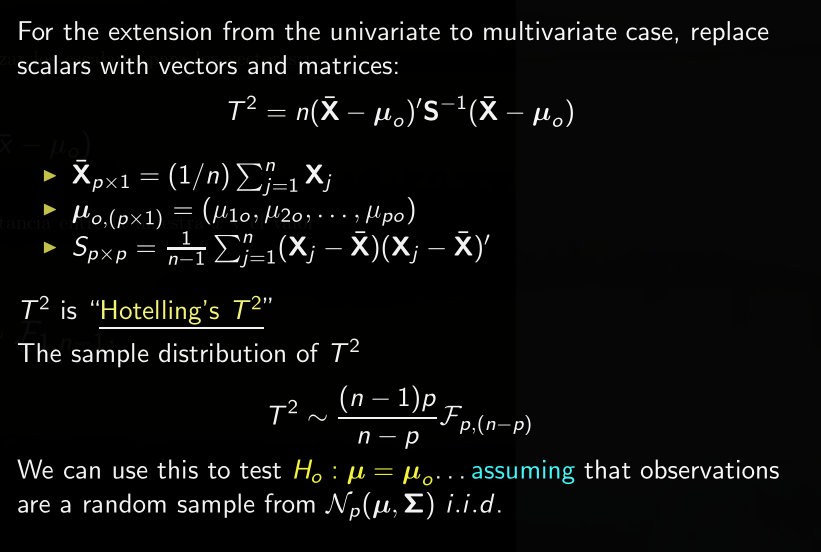
\includegraphics[width=0.8\linewidth]{exten.png}
            \caption{extension al caso multivariado}
            \label{extension al caso multivariado}
        \end{figure}

        hotelingm   $ T ^{2}   $
        \begin{figure}[h!]
            \centering
            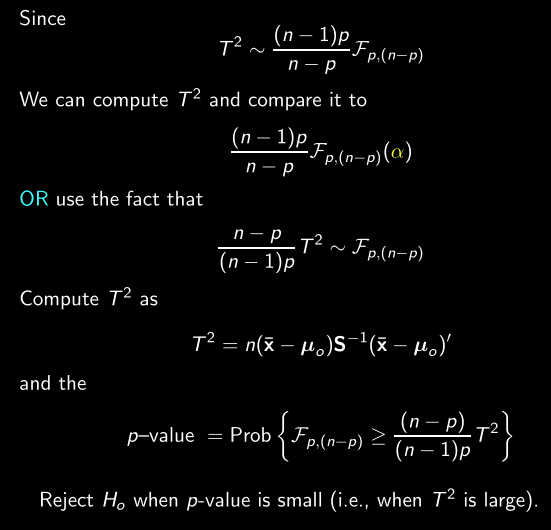
\includegraphics[width=0.8\linewidth]{hoteling.png}
            \caption{Hoteling}
            \label{joteling}
        \end{figure}

        \begin{figure}[h!]
            \centering
            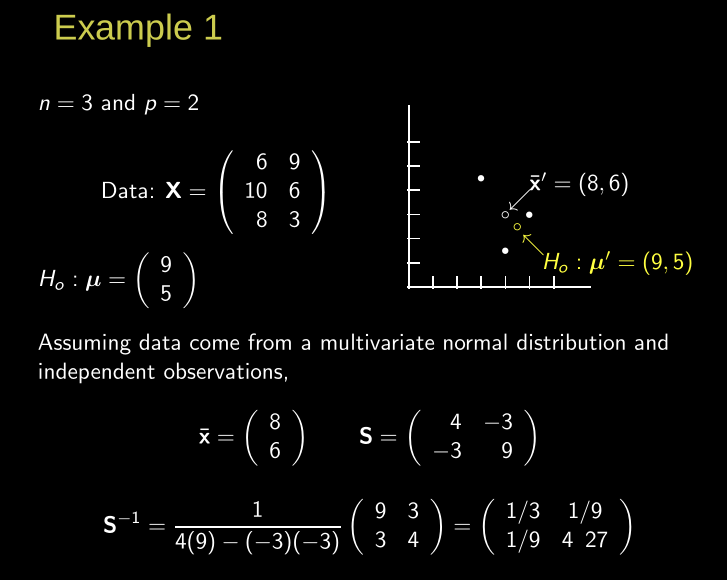
\includegraphics[width=0.8\linewidth]{ejemplo1.png}
            \caption{ejemplo1}
            \label{ejem}
        \end{figure}

        \begin{figure}[h!]
            \centering
            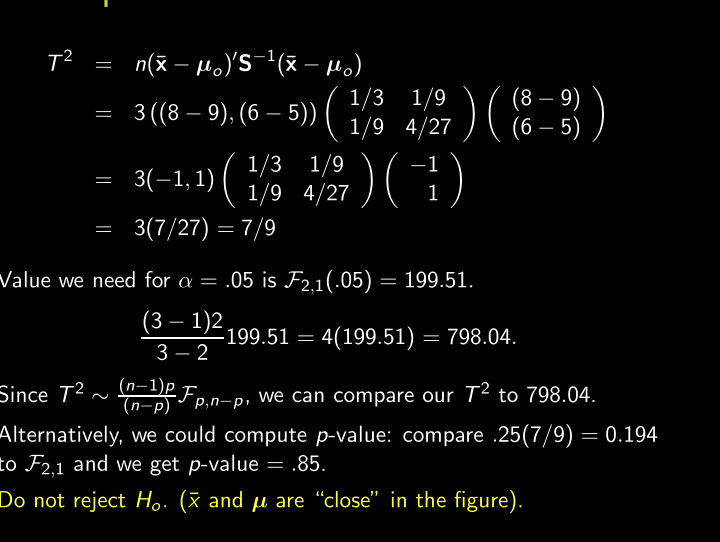
\includegraphics[width=0.8\linewidth]{ejem1.png}
            \caption{ejemplo2 -continuacion}
            \label{ejem}
        \end{figure}

        \color{red} ver el ejemplo 2 y 3\color{white}

    \section{cosas cool}

        \begin{figure}[h!]
            \centering
            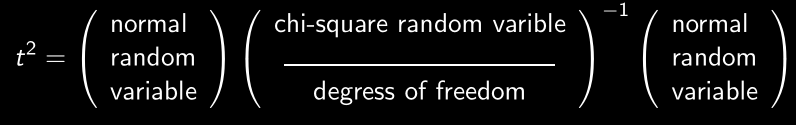
\includegraphics[width=0.8\linewidth]{cool.png}
            \caption{Cosa cool}
            \label{fig}
        \end{figure}


    \section{Likelihood ratio}
        \begin{figure}[h!]
            \centering
            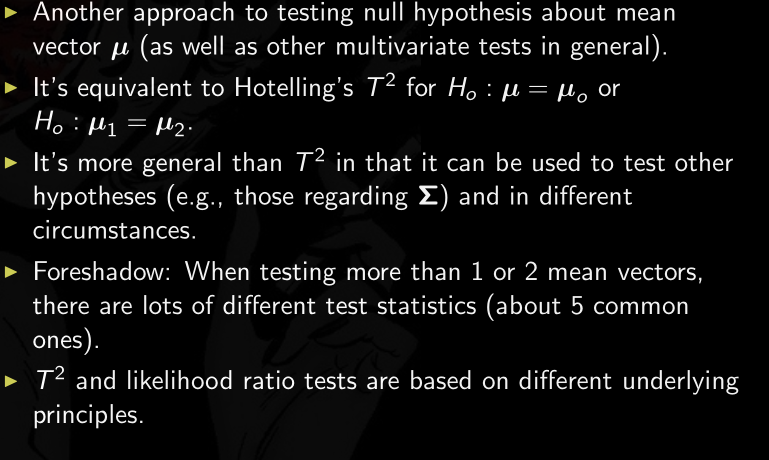
\includegraphics[width=0.8\linewidth]{like.png}
            \caption{Likelihood Ratio }
            \label{fig}
        \end{figure}

        $ T ^{2}   $ esta basado en el principio de la union, que agarra un
        caso multivariado y lo vuelve un problema uniariado, el problema tipo $
        T ^{2} = a'(\hat{X}  - \mu -0)  $  es una combinacion lineal
        \\
        selecionamos el la combinacion del vector que nos lleve al maximo
        posible valor de $ T ^{2}    $ , el plan es ...
        \begin{figure}[h!]
            \centering
            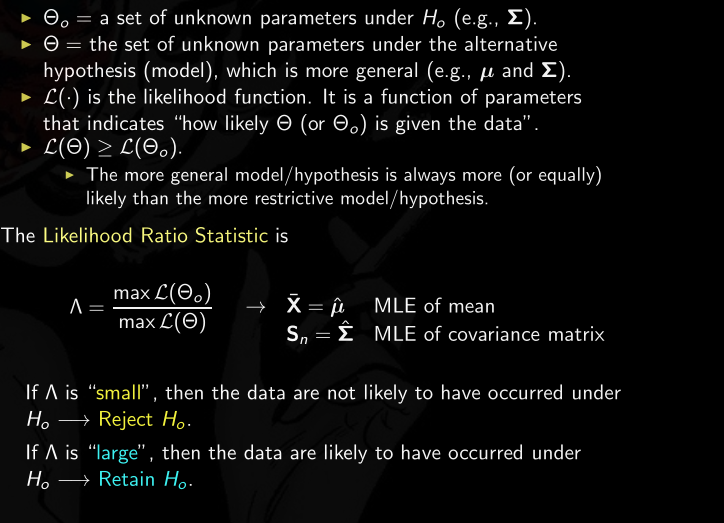
\includegraphics[width=0.8\linewidth]{idea.png}
            \caption{Basic Idea}
            \label{fig}
        \end{figure}

        \begin{figure}[h!]
            \centering
            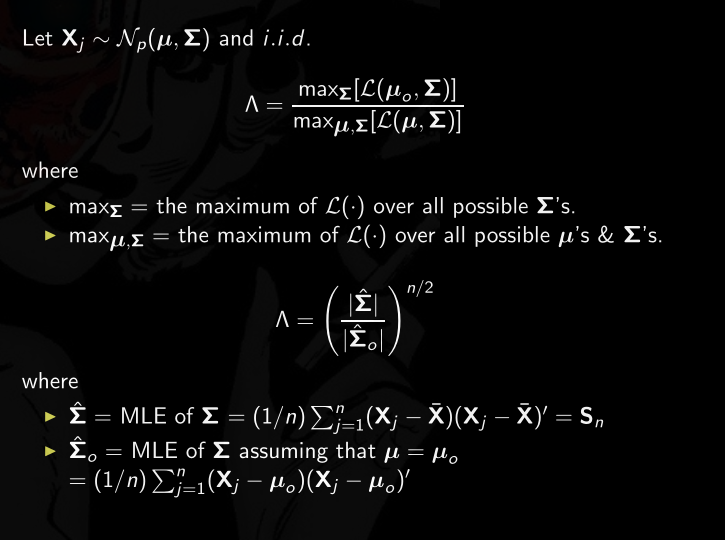
\includegraphics[width=0.8\linewidth]{vectormedias.png}
            \caption{Vector De Medias}
            \label{fig}
        \end{figure}

        \begin{figure}[h!]
            \centering
            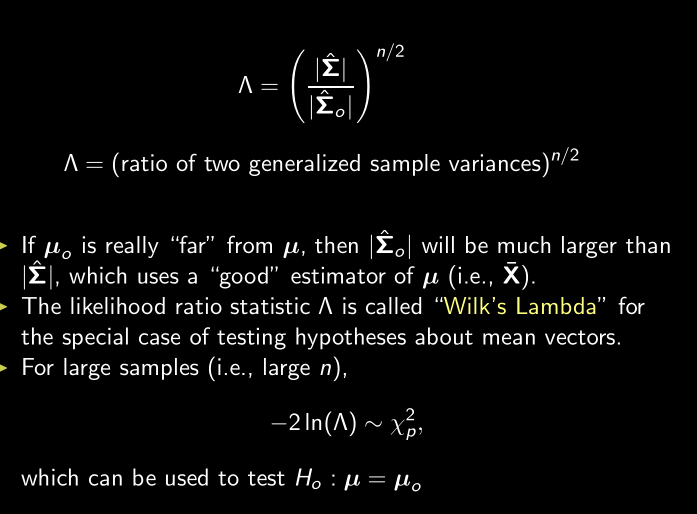
\includegraphics[width=0.8\linewidth]{vecm.png}
            \caption{Vector de medias 2}
            \label{fig}
        \end{figure}

        \begin{figure}[h!]
            \centering
            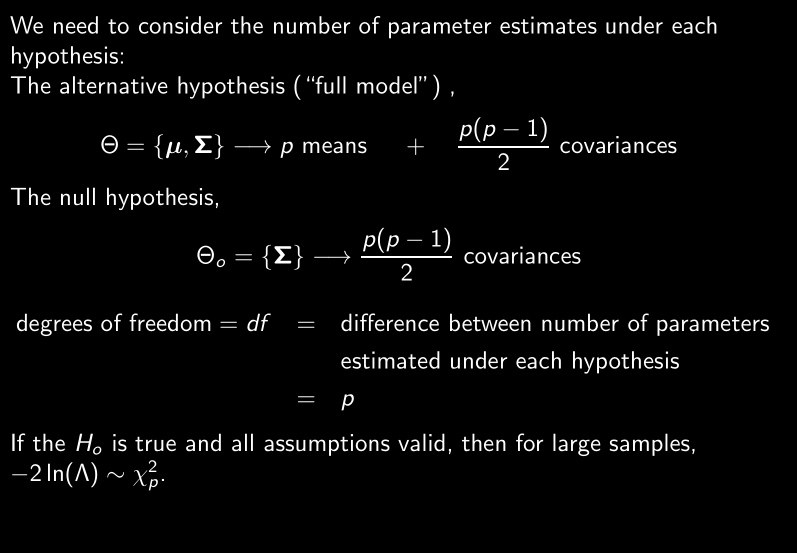
\includegraphics[width=0.8\linewidth]{gradoslibertad.png}
            \caption{Grados de libertad}
            \label{aaaaaa}
        \end{figure}























    %=======================NOTES ENDS HERE===================%

    % bib stuff
    \nocite{*}
    \addtocontents{toc}{{}}
    \addcontentsline{toc}{section}{\refname}
    \bibliographystyle{plain}
    \bibliography{../Bibliography}
\end{document}
